\documentclass[12pt,a4paper]{article}
\title{Lab3-BloomFilter+多线程爬虫}
\usepackage{ctex}
\usepackage{amsmath,amscd,amsbsy,amssymb,latexsym,url,bm,amsthm}
\usepackage{epsfig,graphicx,subfigure}
\usepackage{enumitem,balance}
\usepackage{wrapfig}
\usepackage{mathrsfs,euscript}
\usepackage[usenames]{xcolor}
\usepackage{hyperref}
\usepackage[vlined,ruled,commentsnumbered,linesnumbered]{algorithm2e}
\usepackage{float}
\usepackage{geometry}
\usepackage{listings}
\geometry{a4paper,scale=0.8}

% --- Python code template ---
\usepackage[utf8]{inputenc}
% Default fixed font does not support bold face
\DeclareFixedFont{\ttb}{T1}{txtt}{bx}{n}{12} % for bold
\DeclareFixedFont{\ttm}{T1}{txtt}{m}{n}{12}  % for normal

% Custom colors
\usepackage{color}
\definecolor{deepblue}{rgb}{0,0,0.5}
\definecolor{deepred}{rgb}{0.6,0,0}
\definecolor{deepgreen}{rgb}{0,0.5,0}

\usepackage{listings}

% Python style for highlighting
\newcommand\pythonstyle{\lstset{
language=Python,
basicstyle=\ttm,
morekeywords={self},              % Add keywords here
keywordstyle=\ttb\color{deepblue},
emph={MyClass,__init__},          % Custom highlighting
emphstyle=\ttb\color{deepred},    % Custom highlighting style
stringstyle=\color{deepgreen},
frame=tb,                         % Any extra options here
showstringspaces=false
}}
% Python environment
\lstnewenvironment{python}[1][]
{
\pythonstyle
\lstset{#1}
}
{}

% Python for external files
\newcommand\pythonexternal[2][]{{
\pythonstyle
\lstinputlisting[#1]{#2}}}

% Python for inline
\newcommand\pythoninline[1]{{\pythonstyle\lstinline!#1!}}

% --- Python code template ---


\title{Lab3 \quad BloomFilter+多线程爬虫}
\date{2021.10}
\author{孙济宸\quad \quad 学号:520030910016 \quad  \quad 班级:F2003003}
\begin{document}
\maketitle
\section{实验概览}
\begin{enumerate}
	\item 利用一些hash算法实现BloomFilter数据结构
	\item 使用多线程加速Lab2中对网页的爬取,并用(1)中的BloomFilter加速url查找判重。
\end{enumerate}
\section{实验环境}
\begin{itemize}
	\item Docker
	\item beautifulsoup (bs4)
	\item urllib, urllib.parse, urllib.request
	\item re
	\item hashlib
	\item BKDRHash(提供的代码实现)
\end{itemize}
\newpage

\section{练习题的解决思路}
\subsection{问题1-BloomFilter}
\subsubsection{BloomFilter实现}
初始化:
根据BloomFilter数据结构的算法,首先需要生成k个不同的哈希函数。
哈希函数选择方面,使用了BKDRHash,因为能够方便地生成多组seed。
\\ e.g. k = 7,  BKDRseeds: [31, 131, 1313, 13131, 131313, 1313131, 13131313]\\
最后初始化一个给定长度的bitArray。\\
添加:
\begin{python}
def add(self,str):
        if self.find(str):  #已经存在了,不要再往里加
            return
        for i in range(self.k):     # 将k个哈希函数得到的k位都置为1
            setbit = BKDRHash_withseed(str,self.hashseeds[i]) % self.size   
            # 将hash结果映射到0~k-1
            self.bits.set(setbit)	 #将第setbit位置为1
\end{python}
查询:
\begin{python} 
    def find(self,str):
        for i in range(self.k):
            getbit = BKDRHash_withseed(str,self.hashseeds[i]) % self.size	# 将hash结果映射到0~k-1
            if not self.bits.get(getbit):  
            # 有一bit不匹配,字符串一定不在bloomfilter中
                return False
        return True 
\end{python}
\subsubsection{BloomFilter测试}
首先从字符串集中随机选取testSize个字符串作为测试集;接着创建BloomFilter和作为对照组的set(python标准库)。其中,BloomFilter的参数为bitArray大小和k(哈希函数数量),最优的k用$k_{optimal} = \lceil \ln{2} \frac{m}{n} \rceil$计算得出。
将每个字符串分别加入BloomFilter和set,如果加入时BloomFilter认为字符串已经存在,但是在set中不存在,则说明BloomFilter出现了错误(FalsePositive)。
统计得到的FalsePositive总数量占测试集大小即为错误率(FalsePositiveRate)。
\subsection{问题2-多线程爬虫}
外部IO思路与lab2相同,多线程实现类似BFS,区别是多个线程同时往队列中添加task和获取task。queue中存储的是待爬的url。
先把起始url加入queue,并且设置多个守护线程开始工作。\\
伪代码:\\
\begin{lstlisting}
q: Tasks Queue
crawled: BloomFilter
count: total crawled URLs
def crawl():
    while True:
        page = Top of q
        if page not found in crawled:
           Try getting page, if failed:  call q.task_done()
           
            add_page_to_folder(page, content)
            outlinks = get_all_links(content, page)
           Add all outlinks to q, unless count > maxCount
		  Acquire lock and add page into crawled      
        q.task_done()
        
# main():
Add seed URL  to q
Create some daemon threads to crawl
Wait for all task to be done
\end{lstlisting}
\section{代码运行结果}
\subsection{问题1(BloomFilter)结果}
完整结果见txt文件
\begin{figure}[H]
%	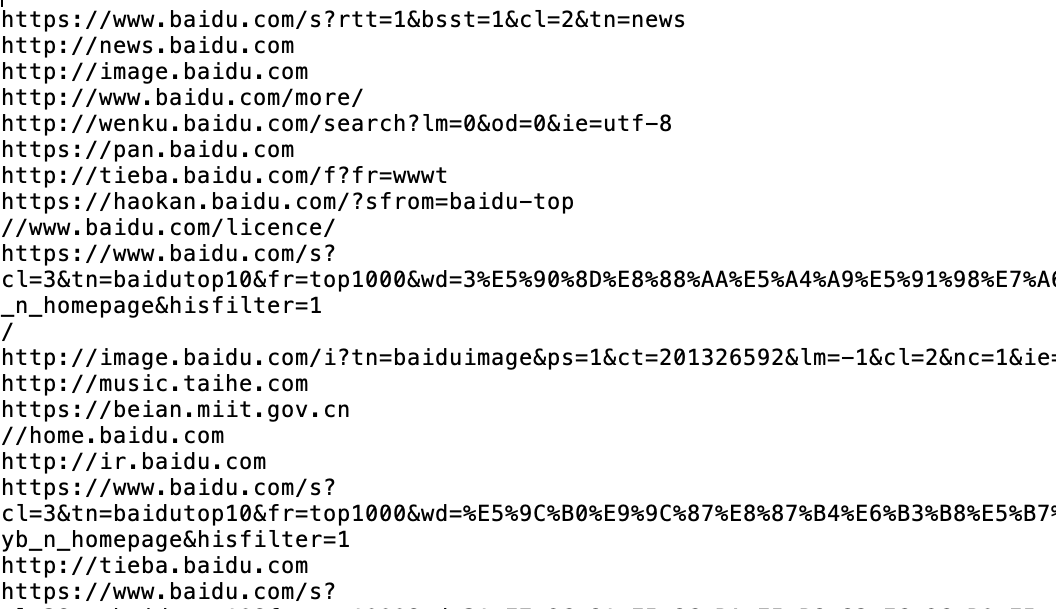
\includegraphics[scale=0.7]{res1.png}
	 \caption{res1.txt}
\end{figure}

\subsection{问题2(多线程爬虫)结果}
\begin{figure}[H]
%	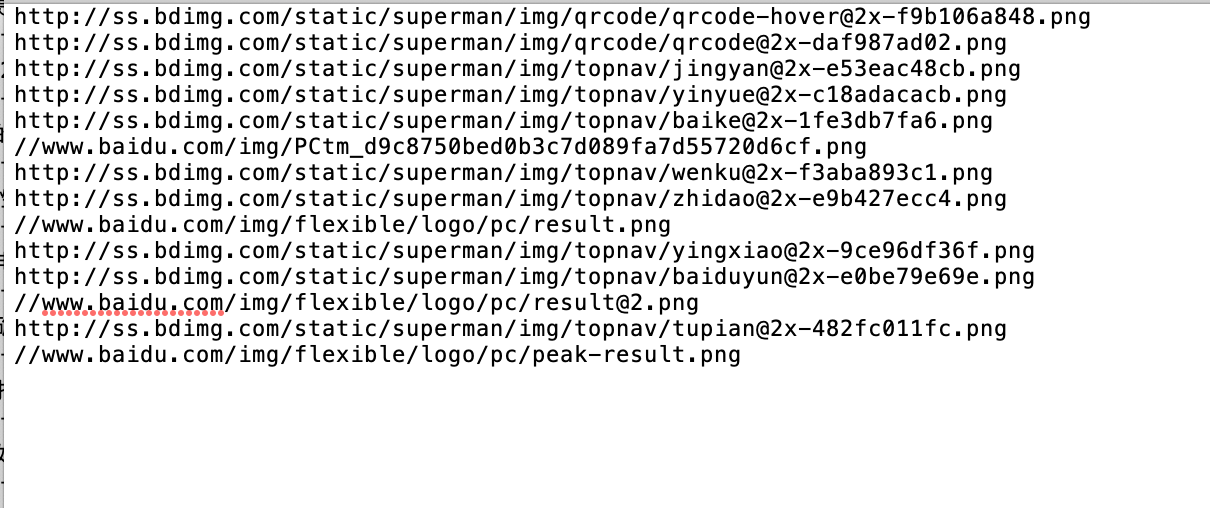
\includegraphics[scale=0.7]{res2.png}
	 \caption{res2.txt}
\end{figure}



\section{分析与思考}
\begin{itemize}
	\item beautifulsoup解析html文件得到的是bs4.BeautifulSoup类型对象; 解析方法如果不指定features = "html.parser",会弹warning。网上资料显示这是默认的解析方法,还可以选择其他的解析方法。
	\item soup.findAll()方法得到一个存有许多标签(tag)的list。这些tag常常是多层嵌套的,可以用parent,contents等多种方法访问。
	\item \textbf{拓展思考:} 问题1中的href url有绝对路径、相对路径和javascript。如果需要进一步处理可能需要分类
	\item tag.find()方法会从这个标签的所有\textbf{子标签}中查找指定内容,并不能查找该标签同层(\textbf{包括自己})的内容!所以问题3中用i.contents[0].find(...)会什么也找不到。这里被坑了好久
	\item 知乎日报文章的标题\textbf{并没有}使用<title>标签,而是用了<span class="title">标签,所以不能直接用tag.title,因此我选择使用tag.string获取标题内容。
\end{itemize}
\end{document}

